\documentclass[../thesis.tex]{subfiles}

\begin{document}

Για την ταυτοποίηση των χρηστών είναι απαραίτητη η επικοινωνία της εφαρμογής με το σύστημα ταυτοποίησης του Πολυτεχνείου, το οποίο βασίζεται στο πρωτόκολλο SAML\footnote{Το SAML (Security Assertion Markup Language) είναι ένα σύστημα σχεδιασμένο για την ασφαλή ανταλλαγή ισχυρισμών (assertions) που αφορούν την ταυτότητα και τις εξουσιοδοτήσεις ενός χρήστη}.
Αντί να επικοινωνούμε απευθείας με τον Identity Provider της σχολής, εκτελούμε την ταυτοποίηση μέσω ενός server Keycloak\footnote{Ο server Keycloak δημιουργήθηκε από τους φοιτητές της σχολής Άγγελο Κολαΐτη και Σταμάτη Κατσιαούνη-Μολυβά } ο οποίος είναι ρυθμισμένος έτσι ώστε να λειτουργεί ως Identity Broker εκ μέρους του.
\todo{Find out who to credit for Keycloak server}
Χρησιμοποιώντας το Keycloak η ταυτοποίηση μπορεί να γίνει μέσω του πρωτοκόλλου OpenID Connect το οποίο είναι πιο εύκολα υλοποιήσιμο από το SAML σε μοντέρνες εφαρμογές.

\subsection*{OAuth και OpenID Connect}
Ο όρος authentication αφορά την ταυτοποίηση ενός χρήστη, ενώ το authorization αφορά μόνο την παροχή άδειας σε μία υπηρεσία για την πρόσβαση σε προστατευμένους πόρους εκ μέρους του χρήστη.
Οι δύο έννοιες είναι στενά συνδεδεμένες, ωστόσο είναι σημαντικό να μη συγχέονται.
Οι προδιαγραφές του OAuth 2.0 δημοσιεύθηκαν τον Οκτώβριο του 2012 από τον οργανισμό IETF (Internet Engineering Task Force) ως επικαιροποίηση των προδιαγραφών του πρωτοκόλλου OAuth 1.0 που είχε δημοσιευθεί το 2007, και γρήγορα υιοθετήθηκαν από πολλές υπηρεσίες του διαδικτύου.
Παρά το γεγονός ότι το OAuth αποτελεί αυστηρά πρωτόκολλο authorization και δεν είναι σχεδιασμένο για authentication, από την απαρχή του το OAuth χρησιμοποιήθηκε καταχρηστικά για το authentication χρηστών από μεγάλο μέρος του διαδικτύου.
Αυτή η λανθασμένη χρήση του OAuth για authentication παρουσιάζει κινδύνους για την ασφάλεια των δεδομένων του χρήστη\cite{oauth_net}.

Το OpenID Connect (OIDC) είναι ένα πρωτόκολλο σχεδιασμένο ειδικά για ασφαλή authentication χρηστών.
Δημοσιεύτηκε το 2014 ως βελτίωση του παλαιότερου πρωτοκόλλου OpenID 1.0/2.0, και βασίζεται πάνω στο authorization framework του OAuth 2.0.
Το OIDC παρουσιάζει μία μέθοδο ταυτοποίησης η οποία είναι συμβατή με το ήδη εδραιωμένο πρωτόκολλο OAuth 2.0, επιτρέποντας την εύκολη υλοποίηση του authentication τόσο από πλευράς του Identity Provider όσο και από πλευράς του Client\cite{oidc_faq}.

\begin{figure}[!ht]
    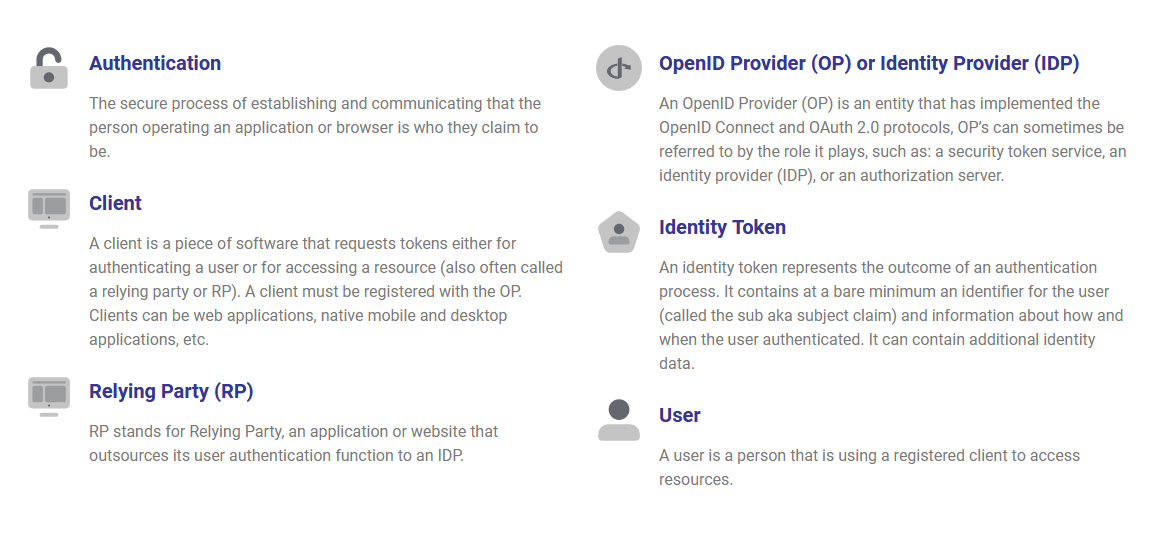
\includegraphics[width=\textwidth]{oidc_definitions.png}
    \centering
    \caption{Ορισμοί των βασικών όρων που χρησιμοποιούνται στο πρωτόκολλο OpenID Connect\cite{oidc_faq}.}
\end{figure}

Θα περιγράψουμε συνοπτικά τη διαδικασία ταυτοποίησης που γίνεται για την πρόσβαση των στοιχείων του χρήστη από την ιστοσελίδα της εφαρμογής μέσω του browser.
Η υλοποίηση της περιγράφεται παρακάτω στην ενότητα \hyperref[sec:website]{Ιστοσελίδα}.
Η ροή ταυτοποίησης ξεκινάει όταν ο χρήστης ζητήσει πρόσβαση στον πόρο που απαιτεί δικαιώματα πρόσβασης, δηλαδή στη σελίδα του προφίλ του.
Ο web server δέχεται το αίτημα και ελέγχει αν ο συγκεκριμένος χρήστης είναι ήδη συνδεδεμένος.
Αν όχι, τότε ξεκινάει το λεγόμενο authorization code flow που ορίζεται από το πρωτόκολλο OpenID Connect για την ταυτοποίηση του χρήστη.
Ο server (Relying Party) ανακατευθύνει τον browser του χρήστη στην ιστοσελίδα του Keycloak (Identity Provider) με τις κατάλληλες παραμέτρους που προσδιορίζουν το αίτημα (client ID/secret, redirect URI, code challenge κ.ά.).
Αφού ο χρήστης εισάγει τα στοιχεία του, το Keycloak ανακατευθύνει με τη σειρά του τον browser πίσω στην ιστοσελίδα του server, περιλαμβάνοντας στις παραμέτρους του συνδέσμου έναν κώδικα που δίνει πρόσβαση στα στοιχεία του χρήστη.
Μόλις ο server λάβει την αίτηση αυτή από τον χρήστη, παρουσιάζει τον κώδικα στο Keycloak, το οποίο τελικά του προσφέρει τα στοιχεία του χρήστη με τη μορφή JWT.
Σε αυτό το σημείο ο server επαληθεύει την εγκυρότητα του token, και αφού εξάγει τις πληροφορίες που χρειάζεται (στην περίπτωσή μας τον ΑΜ και ονοματεπώνυμο) τις αποθηκεύει στο session του χρήστη.
Από το σημείο αυτό και πέρα, κάθε αίτημα του χρήστη προς τον server συνοδεύεται από ένα session cookie το οποίο ο server μπορεί να χρησιμοποιήσει για να αντιστοιχίσει το αίτημα του χρήστη με το κατάλληλο session, και επομένως με την ταυτότητα του.

\begin{figure}[!ht]
    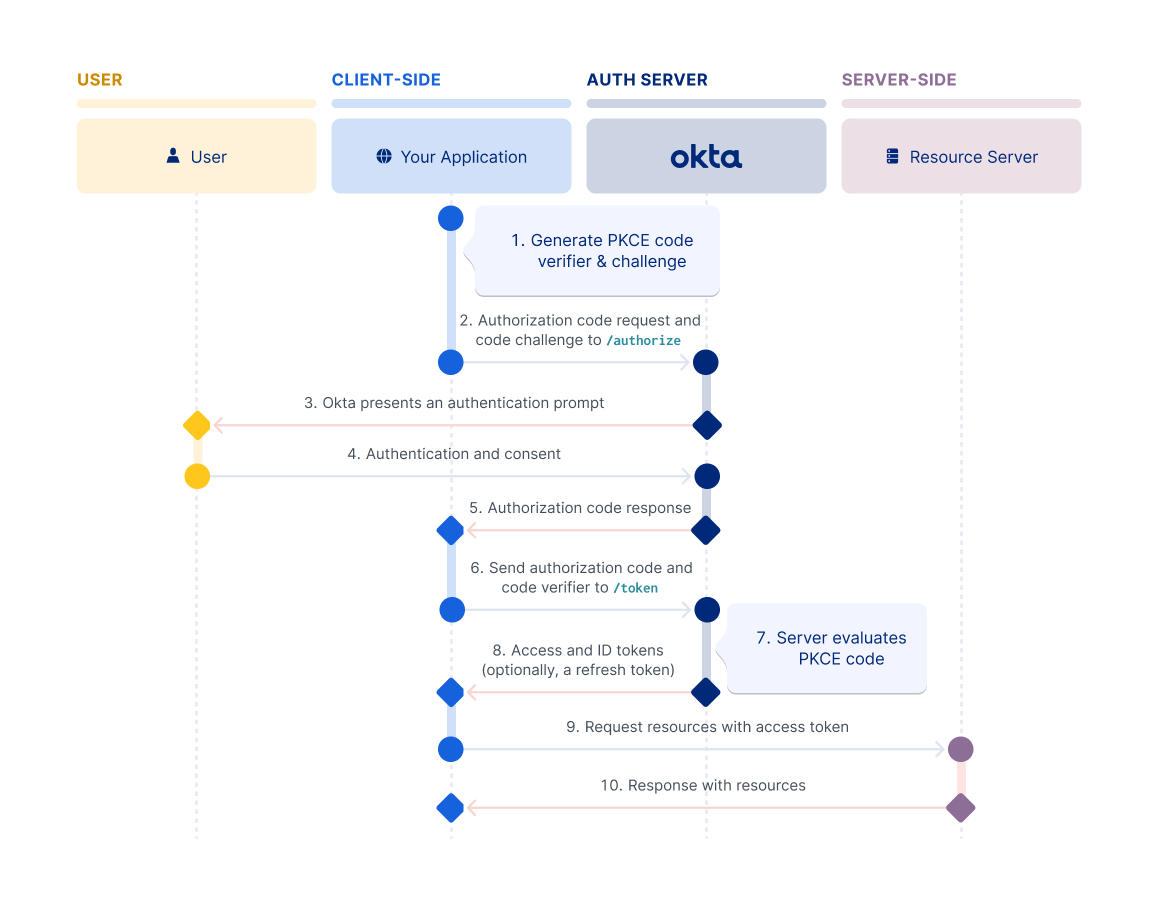
\includegraphics[width=\textwidth]{oauth_code_flow}
    \centering
    \caption{Το authorization code flow σε περισσότερη λεπτομέρεια. Στην περίπτωσή μας ο \textit{client} είναι ο server, και ο \textit{auth server} είναι το Keycloak. H διαδικασία σταματάει στο βήμα 8 καθώς μας ενδιαφέρει μόνο το ID Token το οποίο ταυτοποιεί τον χρήστη, και δε χρειαζόμαστε το access token για πρόσβαση σε εξωτερικό API/\textit{resource server}\cite{okta_code_flow}.}
\end{figure}

Το authentication του χρήστη στην εφαρμογή κινητού λειτουργεί με παρόμοιο τρόπο, με τη διαφορά ότι ο \textit{client} είναι πια εφαρμογή κινητού και όχι browser, γεγονός που σημαίνει ότι απαιτείται ειδική μέριμνα για την προστασία των προσωπικών στοιχείων του χρήστη.
Για τον σκοπό αυτό συστήνεται η χρήση του AppAuth, μίας βιβλιοθήκης που δημιουργήθηκε από την OpenID Foundation για authentication εντός κινητών εφαρμογών.
Το βασικό σημείο που χρήζει προσοχής είναι η επικινδυνότητα της χρήσης \textit{embedded user-agent} και συγκεκριμένα των in-app webviews στη διαδικασία ταυτοποίησης.
Τα webviews χρησιμοποιούνται εκτεταμένα σε κινητές εφαρμογές καθώς επιτρέπουν τη φόρτωση ιστοσελίδων εντός της εφαρμογής, παρέχοντας αυξημένο έλεγχο στην εμφάνιση και στη λειτουργία του "browser".
Αυτές όμως οι δυνατότητες που προσφέρουν τα webviews τα καθιστούν πλέον ακατάλληλα για authentication, καθώς η εφαρμογή έχει πλήρη πρόσβαση στα στοιχεία σύνδεσης που ο χρήστης εισάγει στη φόρμα ταυτοποίησης.\cite[\S8.12]{rfc8252}
Για αυτόν τον λόγο το AppAuth χρησιμοποιεί εξ ολοκλήρου τον αξιόπιστο default system browser του χρήστη\footnote{Safari στις συσκευές iOS, και Google Chrome στις συσκευές Android} για το authentication flow, επιστρέφοντας στο τέλος της διαδικασίας μόνο το authorization code στην εφαρμογή.
Έτσι προστατευόμαστε από πιθανούς κινδύνους ασφαλείας που εγκυμονούν τα webviews, και διατηρείται η εμπιστοσύνη του χρήστη στην ασφάλεια της εφαρμογής.
Τέλος, ο εξωτερικός browser διατηρεί όλους τους αποθηκευμένους κωδικούς και τα sessions του χρήστη, διευκολύνοντας τη σύνδεση του στην εφαρμογή και επομένως βελτιώνοντας την εμπειρία του.

Στην εφαρμογή η κλάση \verb|Authenticator| είναι υπεύθυνη για το authentication.
Η κλάση χρησιμοποιεί το plugin \verb|FlutterAppAuth| το οποίο υλοποιεί το πρωτόκολλο AppAuth σε όλες τις πλατφόρμες, και εκτελεί τις μεθόδους \verb|authenticate| και \verb|endSession|.

\begin{codeblock}{dart}{authenticator.dart}
  class Authenticator {
    const appAuth = FlutterAppAuth();
    String? _idToken;

    String? get idToken => _idToken;
  
    Future<String?> authenticate() async {
      final request = AuthorizationTokenRequest(
        authClientID,
        '\$appScheme:/auth',
        issuer: authIssuer,
        scopes: ['openid', 'profile', 'email'],
        additionalParameters: {'kc_idp_hint': 'saml'},
      );
      final response = await appAuth.authorizeAndExchangeCode(request);
      _idToken = response?.idToken;
      return _idToken;
    }
  
    Future<EndSessionResponse?> endSession() {
      final request = EndSessionRequest(
        issuer: authIssuer,
        idTokenHint: _idToken,
        postLogoutRedirectUrl: '\$appScheme:/',
      );
      final response = await appAuth.endSession(request);
      if (response != null) _idToken = null;
      return response;
    }
  }  
\end{codeblock}

Η μέθοδος authenticate στέλνει το authorization request με τις κατάλληλες παραμέτρους στον Identity Provider της σχολής, και λαμβάνει το ID Token το οποίο επιστρέφεται στην εφαρμογή και τελικά στέλνεται στον server για την έναρξη της σύνδεσης.
Με παρόμοιο τρόπο η μέθοδος endSession στέλνει το end session request στον IDP και ακυρώνει το υπάρχον ID Token, λήγοντας τη σύνδεση με τον server.
Αξιοσημείωτη είναι η χρήση του appScheme στο πεδίο του redirectUri.
Το appScheme\footnote{Το app scheme της εφαρμογής μας είναι το "gr.ntua.ece.ridehailing" σύμφωνα με το reverse domain naming convention} αποτελεί το αναγνωριστικό της εφαρμογής, και η χρήση του ως redirect URI σημαίνει ότι μόλις ολοκληρωθεί η ταυτοποίηση στον IDP, ο χρήστης θα μεταβεί αυτόματα πίσω στην εφαρμογή όπως περιγράψαμε προηγουμένως.

Από την πλευρά του server, το JSON Web Token λαμβάνεται μέσα από τα headers του request, και αποκωδικοποιείται/επαληθεύεται.
Αν το JWT είναι έγκυρο τότε επιστρέφεται ένα αντικείμενο με τα σχετικά στοιχεία του χρήστη και ο server μπορεί να προχωρήσει στη ρύθμιση της σύνδεσης.

\begin{codeblock}{typescript}{api.ts/authenticate}
  async function authenticate(req: IncomingMessage) {
    let idToken = req.headers["authentication"];
    loggerTraffic.info(`Connection attempted`);
    if (!idToken) return;
    let decodedToken;
    try {
      decodedToken = (await jwtVerify(idToken, JWKS)).payload;
    } catch (error) {
      loggerMain.warn(error);
      return;
    }
    if (!decodedToken || !decodedToken.name || !decodedToken.id) {
      loggerMain.warn(
        `Client tried to connect with invalid info: ` +
          JSON.stringify(decodedToken, null, 2)
      );
      return;
    }
    return {
      id: decodedToken.id as string,
      full_name: decodedToken.name as string,
    } as Credentials;
  }
\end{codeblock}

\end{document}